%! Author = zero
%! Date = 29/07/2024

% Preamble
\documentclass[a4paper, 12pt]{article}

\usepackage[english,russian]{babel}
\usepackage[T2A]{fontenc}
\usepackage[utf8]{inputenc}
\usepackage{geometry}
\usepackage{enumitem}
\usepackage{setspace}
\usepackage{amssymb}
\usepackage{graphicx}
\usepackage{float}
\usepackage{wrapfig}
\geometry{top=5mm}
\renewcommand{\arraystretch}{1.2}
\linespread{1}

% Document
\begin{document}
    \begin{center}
        \textbf{
            Самостоятельная работа №2\\
            Основы алгебры логики}
    \end{center}

    \begin{center}
        \textbf{№1 Найти значения: $\textbf{C, D, E, F}$, если $\textbf{A = 0, B = 1}$}
    \end{center}

    Ответ: $C = 1, D = 1, E = 1, F = 0$

    \begin{center}
        \textbf{№2 Построить таблицу истинности:}
    \end{center}

    \begin{minipage}[t]{0.4\textwidth}
        \begin{enumerate}
            \begin{spacing}{0.5}
                \item $A \vee B \wedge \overline B$\\
            \end{spacing}
            \begin{tabular}{|c|c|c|}
                \hline
                $A$ & $B$ & $F$ \\
                \hline
                $0$ & $0$ & $0$ \\
                \hline
                $0$ & $1$ & $0$ \\
                \hline
                $1$ & $0$ & $1$ \\
                \hline
                $1$ & $1$ & $1$ \\
                \hline
            \end{tabular}
        \end{enumerate}
    \end{minipage}
    \begin{minipage}[t]{0.4\textwidth}
        \begin{enumerate}
            \setcounter{enumi}{1}
            \begin{spacing}{0.5}
                \item $(B \vee C) \wedge (\overline A \wedge C \vee \overline C)$\\
            \end{spacing}
            \begin{tabular}{|c|c|c|c|}
                \hline
                $A$ & $B$ & $C$ & $F$ \\
                \hline
                $0$ & $0$ & $1$ & $1$ \\
                \hline
                $0$ & $1$ & $0$ & $1$ \\
                \hline
                $0$ & $1$ & $1$ & $1$ \\
                \hline
                $1$ & $0$ & $0$ & $0$ \\
                \hline
                $1$ & $0$ & $1$ & $0$ \\
                \hline
                $1$ & $1$ & $0$ & $1$ \\
                \hline
                $1$ & $1$ & $1$ & $0$ \\
                \hline
            \end{tabular}
        \end{enumerate}
    \end{minipage}

    \begin{center}
        \textbf{№3 Решить кругами Эйлера:}
    \end{center}

    \begin{minipage}[t]{0.4\textwidth}
        \centering
        \begin{enumerate}
            \item $A \wedge B \vee C$\\
            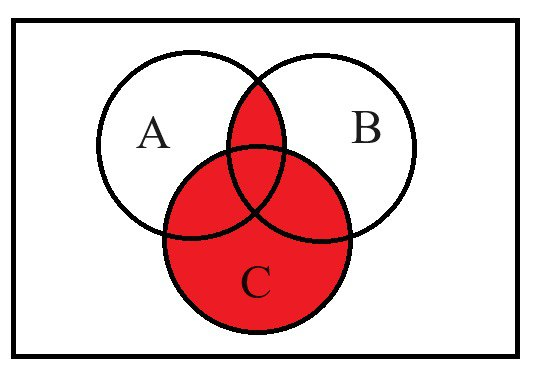
\includegraphics[width=1\linewidth]{images/im1}
        \end{enumerate}
    \end{minipage}
    \begin{minipage}[t]{0.4\textwidth}
        \centering
        \begin{enumerate}
            \setcounter{enumi}{1}
            \item $Z \vee A \wedge C \vee \overline B$\\
            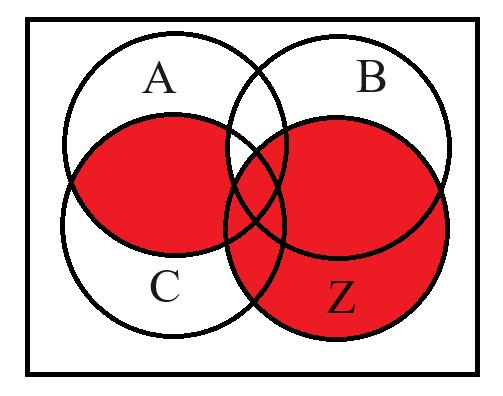
\includegraphics[width=1\linewidth]{images/im2}

        \end{enumerate}
    \end{minipage}

    \begin{center}
        \textbf{№4 Решить уравнение:}
    \end{center}

    \begin{tabular}{|c|c|c|c|c|}
        \hline
        $X$ & $Y$ & $X \wedge Y$ & $X \wedge Y \vee Y$ \\
        \hline
        $0$ & $0$ & $0$          & $0$                 \\
        \hline
        $0$ & $1$ & $0$          & $1$                 \\
        \hline
        $1$ & $0$ & $0$          & $0$                 \\
        \hline
        $1$ & $1$ & $1$          & $1$                 \\
        \hline
    \end{tabular}
    Ответ: (0, 1), (1, 1)

\end{document}